\chapter{Data fusion problem formulation}\label{ch:02DataFusionProblem}
\noindent For each point $\vec{p}\in\R^3$ in space there is set of questions which can be asked:

\begin{enumerate}
    \item \emph{Is point visible ?} - how good can be point or space partition observed during vehicle flight before decision.
    \item \emph{Is there obstacle ?} - how sure I can be that there is observation of obstacle.
    \item \emph{Is point reachable ?} - how is maximum safety of any route leading to given point.
\end{enumerate}
\noindent To address these issues it is necessary to identify related ratings and bound them to space representation artifacts. In this case we have two space representation merged together in one avoidance grid $\mathscr{A}(t_i)$:
\begin{enumerate}
    \item\emph{Cells $c_{i,j,k}$} belongs to planar space $c_{i,j,k}\in\R^3$ and represents a set of points bounded by cell, the ratings bounded to cells are representing \emph{visible space assessment}.
    \item\emph{Trajectories $\mathscr{T}(\vec{x}_0,B)$} belongs to vehicle system state space $\mathscr{T}(\vec{x}_0,B)\in\R^n$, where $n\in\N^{3+}$ and there exist projection function $\mathscr{P}:\R^{n}\to\R^3$ which projects vehicle trajectory $\mathscr{T}(\vec{x}_0,B)$ to visible space $\R^3$, the ratings bounded to trajectories are representing \emph{state space assessment}
\end{enumerate}
\noindent \emph{State space assessment} and \emph{visible space assessment} are interconnected and the ratings are impacting each other between spaces. The final value of the particular rating is given by \emph{general algorithm}.
\section{Deterministic approach shortcomings}\label{sec:deterministicApproachShortcommings}
\noindent This subsection contains identified shortcomings of \emph{deterministic approach}. The identified shortcomings varies trough different topics and their impact is reviewed in terms of probabilistic approach.

\subsection{Changing scanning density of LiDAR}
\noindent LiDAR is scanning in conic section given by $d_r,\theta_r,\varphi_r$, where $d_r$ is distance range, $\theta=[s,e],s,e\in [0,2\pi]$ is horizontal rotation range, and $\varphi=[s,e] s,e\in[0,\pi/2]$ is vertical offset range. Let say that $d\theta, d\varphi$ is unitary angle offset in which one LiDAR send and return is executed. The surface of area given by some distance d, and unitary offsets $d\theta, d\varphi$ is changing with $d$. The area of tresholding object surface is not changing. This fact has an impact on count of the hits on some surface. The example is given in fig. \ref{fig:P01CountOfLiDARHits} where we have two identical objects (red circle) in distances 5 and 10 meters. The closer object consumes 5 LiDAR beam hits and the farther object consumes only 3 LiDAR beam hits. The probability of obstacle encounter is remaining the same for closer and farther object. \emph{Probabilistic approach must handle this issue} and return the same probability of obstacle collision for objects with same scanned surface (with different LiDAR beam hit count).

\begin{figure}[htbp]
    \centering
    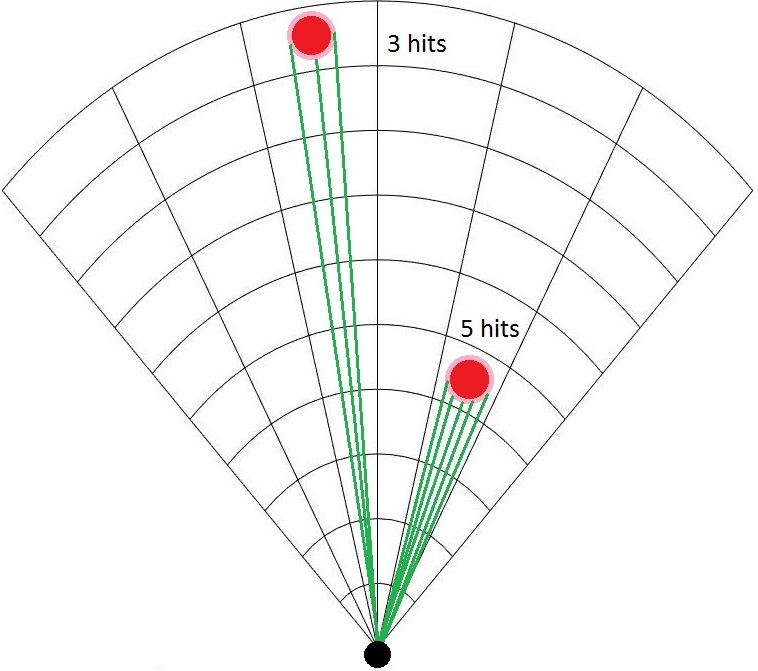
\includegraphics[width=0.7\textwidth]{\FIGDIR/P01CountOfLiDARHits}
    \caption{Different count of LiDAR hits on objects with same size but different distance from vehicle}
    \label{fig:P01CountOfLiDARHits}
\end{figure}

\section{Fusion of obstacle map with detected obstacles}
\noindent The concept of \emph{offline/online obstacle map} is mandatory in modern obstacle avoidance systems and increases the safety of trajectory planning. \emph{Deterministic} concept was considering only LiDAR reading or \emph{real-time reading} in general. The fusion of real time reading and obstacle map (prior knowledge) is required. Data fusion of these two sources is strongly depending on visibility property, because there are three basic scenarios:
\begin{enumerate}
    \item \emph{Dual detection} - the obstacle is marked on the map and detected by sensory system at some point of the time (deterministic concept works).
    \item \emph{Hindered vision} - the detected obstacles are hindering vision to map obstacle therefore map obstacle uncertainty arises (deterministic concept fails). 
    \item \emph{False-positive map} - map obstacle occupied space is visible by sensory system, but negative detection is returned. Therefore the map is giving \emph{false-positive} information.
\end{enumerate}
\noindent The second case is given in fig. \ref{fig:P02OvershadowedMapobstacle}, where map obstacle (blue circle) is overshadowed by three scanned obstacles (red circle). The visible space is denoted by green fill, the invisible space is denoted by gray fill. 


\begin{figure}[htbp]
    \centering
    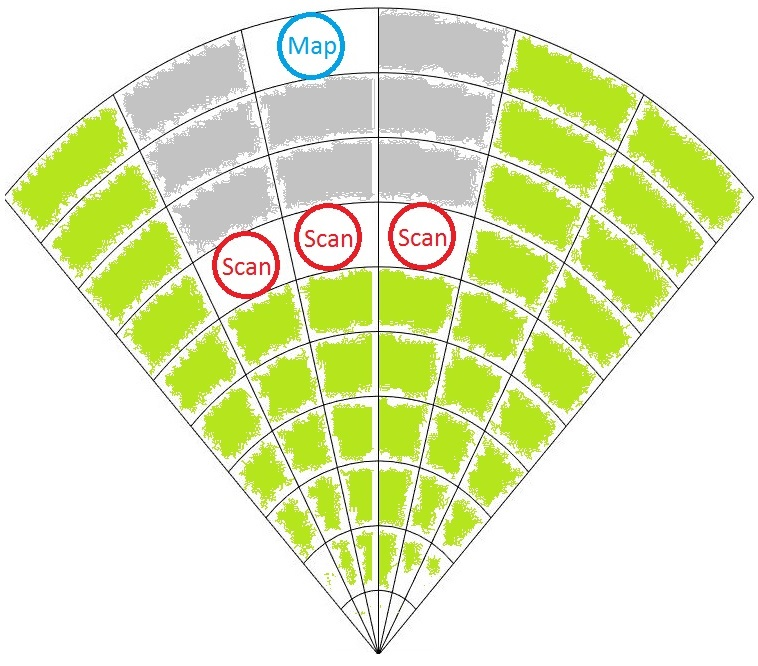
\includegraphics[width=0.7\textwidth]{\FIGDIR/P02OvershadowedMapobstacle}
    \caption{Overshadowed map obstacle by detected obstacles}
    \label{fig:P02OvershadowedMapobstacle}
\end{figure}


\subsection{Adversary/Intruder probability spread}
\noindent \emph{Adversarial behaviour} is first incorporation of moving obstacle. The Adversary is trying to destroy avoiding vehicle. Intruder concept will be used instead of adversary concept in this work. The \emph{intruder} vehicle (for short intruder) is in non-cooperative mode and is not trying to hurt our vehicle. The non-cooperative premise is given by current standard behaviour of small UAV vehicles. \emph{Minimal data set} which can extracted for any intruder consist from:
\begin{enumerate}
    \item\emph{Position} $\vec{p}\in\R^3$ - position of intruder in any transferable vehicle coordinate frame can be extracted and converted into \emph{avoidance coordinate frame}
    \item\emph{Heading (velocity)} $\vec{v}\in\R^3$ - heading with time parameter or velocity of intruder can be read or estimated trough various means. It must be converted into \emph{avoidance coordinate frame}.
    \item\emph{Uncertainty spreads} $\theta,\varphi,\dots$ - various spreads of uncertain intruder maneuverability.
\end{enumerate}

\noindent Example of intruder intersection without \emph{time of intersection} consideration is given in fig. \ref{fig:P03AdversaryProbabilitySpread}. The intruder initial position $\vec{p}$ at time of avoidance $t_i$ is denoted as green circle with 'A' letter. The intruder linear path approximation based on velocity $\vec{v}$ is denoted as middle green line. The spread of intruder maneuverability is given as outer green lines. The probability of intersection is denoted as green-orange-red cell fill, meaning is the red is high probability of intersection, orange is medium probability of intersection and green is low probability of intersection. 

\begin{figure}[htbp]
    \centering
    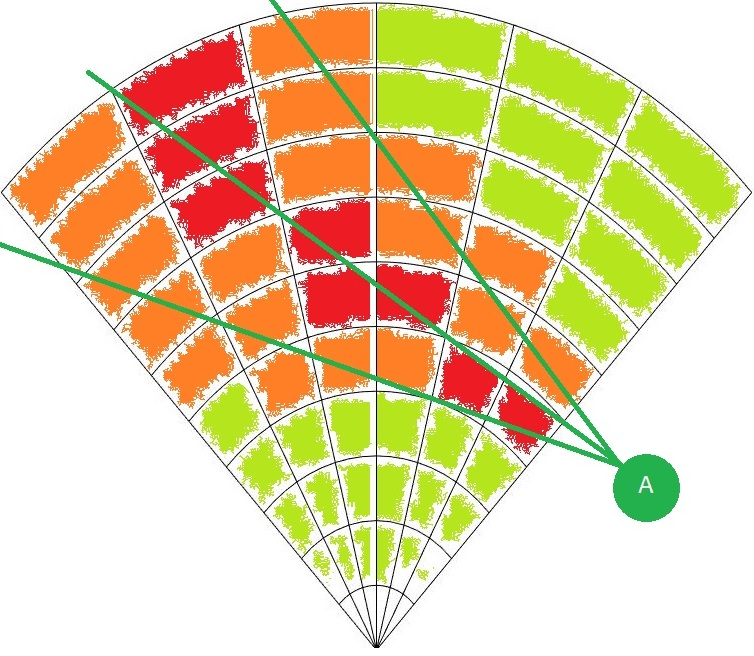
\includegraphics[width=0.7\textwidth]{\FIGDIR/P03AdversaryProbabilitySpread}
    \caption{Intruder vehicle collision probability along assumed trajectory with uncertain spread.}
    \label{fig:P03AdversaryProbabilitySpread}
\end{figure}

\subsection{Safety of passing trajectories}
\noindent Safety of passing trajectories is given by combined safety of passing cells. Each trajectory $\mathscr{T}(\vec{x},B)$ incorporated in reach set approximation $\mathscr{R}(\vec{x},t_i,t_{i+1})$ is passing trough ordered set of cells $\mathscr{C}\subset\mathscr{A}(t_i)$. The base safety rating of single cell $c_{i,j,k}\mathscr{C}$ can be expressed as product of cell visibility rating and inverted cell obstacle rating. Simply if cell is visible and probability of obstacle is low, cell is safe. \emph{Safe trajectory} is trajectory which have safe space along the path. The example of trajectories safety is given in fig. \ref{fig:P04SafetyOfPassingTrajectories}. The safety ratings of cell are given by red-orange-pink-green fills, where red denotes very low safety, orange denotes low safety, pink denotes medium safety, green denotes high safety. Blue trajectory is passing trough many unsafe cells and therefore overall safety is dangerous. Yellow trajectory is passing trough few cells with low and medium safety, therefore the choice of this trajectory is questionable. Green trajectory is passing only trough one cell with medium (pink) cell otherwise it passes trough all very safe cells, therefore its safe to chose this trajectory. The obstacle which caused such cell safety assessment is denoted as black filled circle with 'O' markings.

\begin{figure}[htbp]
    \centering
    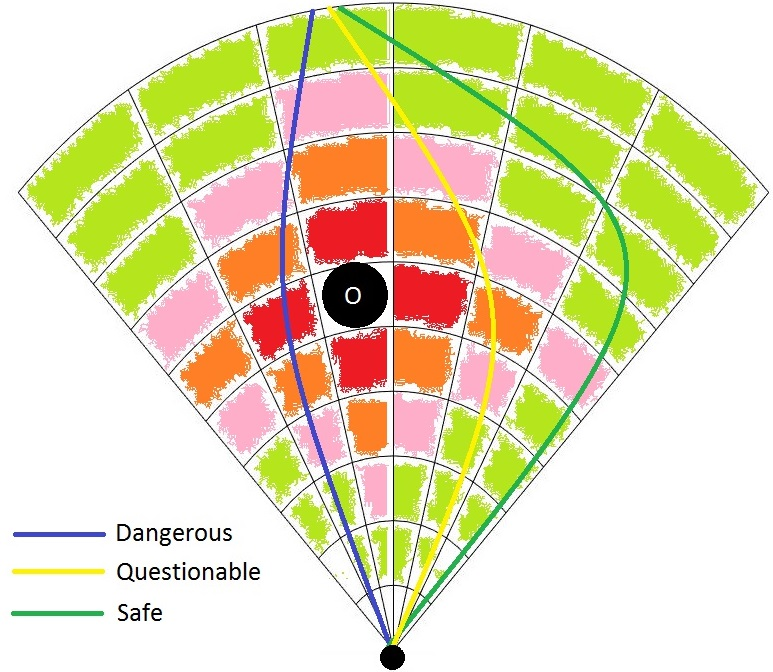
\includegraphics[width=0.7\textwidth]{\FIGDIR/P04SafetyOfPassingTrajectories}
    \caption{Trajectories leading to same destination with different safety ratings.}
    \label{fig:P04SafetyOfPassingTrajectories}
\end{figure}

\subsection{Addressed issues summary}
\noindent Following issues have been extracted of previously mentioned situations. they have been generalized in context of previous \emph{deterministic} approach, offline obstacle map, and intruder behaviour model.

\begin{enumerate}
    \item \textit{Model for intruder passing} - intruder can pass trough vehicle`s FOV at different times with different probability. There are multiple intruder behaviours which have not been accounted in previous approach, like intruder speed and heading uncertainty, intruder own maneuverability etc ...
    \item \textit{Multiple obstacle sources} - concept of visibility is mandatory for map and sensor reading obstacle fusion. The introduction of visibility needs to be done prior multiple source data fusion.
    \item \textit{Reachibility differentiation} - some cells in avoidance grid $\mathscr{A}(t_i)$ are more reachable than other, for example cell with one feasible trajectory has same reachability than cell with multiple leading trajectory.
    \item \textit{Decision making support} - some trajectories leading to same goal have different execution cost and different safety rating, this can be used as additional decision factor. For example framework can choose more expensive but safer trajectory to avoid.
    \item \textit{Obstacle size impact} - obstacle size can have impact on cell safety rating, in deterministic approach cell with one small obstacle have same safety rating than cell with big obstacle.
\end{enumerate}

\newpage
\section{Probabilities for trajectory and grid cell}
\noindent The preliminary analysis of scenarios and identified behaviours and impacts of probabilistic approach gives us an opportunity to identify specific track-able ratings for cell and trajectory artifacts. 
Each cell $c_{i,j,k}$ at avoidance time $t_i$ must have assessed this minimal set of probabilities:
\begin{enumerate}    
    \item \textit{Obstacle probability $P_O$} - determines the probability of obstacle encounter in given cell, obstacle probability is combination of various sources. Initial value of obstacle probability $P_O$ is assumed as 100 \%.
    \item \textit{Visibility $P_V$} -determines visibility of cell at time of avoidance $t_i$, portion of sight into cell space can be hindered by obstacles in front of cell.
    \item \textit{Reachibility $P_R$} - determines the maximum reachability like-hood for given cell based on passing trajectories. 
\end{enumerate}

\noindent Each trajectory $\mathscr{T}(x_0,B)\in\mathscr{R}(t_0,t_1,x_0)$ for each trajectory point $p_\mathscr{T}\in\left\{\mathscr{T}(x_0,B)\to\R^3\right\}$ must have assessed this minimal set of properties: 
\begin{enumerate}    
        \item \textit{Reachibility $P_R$} - determines reachability rating of given point $p_\mathscr{T}$.
        \item \textit{Feasibility of decision $P_D$} - determines next decision feasibility rating.
\end{enumerate}
